\chapter{Methodology}


\section{Introduction}
		Given the average driver's biological senses, they only have a few moments to react upon acknowledging the warning signals from ERs. Within these moments, the drivers must identify the ER's location and heading, understand their maneuver options, and safely execute their plan. Unfortunately, it is common for urban roads to approach over-saturated volume-to-capacity ratios resulting in congestion and little space to maneuver \cite{archer_2005, traffic_data_computation_method_2018}. In these situations, ERs are often upon the drivers (i.e., within 150-meters of them) before the traffic can clear a path, causing chaos and significant delays to reach emergency sites which may have fatal ramifications. As risk can be measured as a relation to exposure to nearby traffic \cite{archer_2005, traffic_data_computation_method_2018}, these increases in traffic volumes around and ahead of ERs constitute a substantial cause for delays when responding to emergencies and increase the risk of other accidents \cite{Hsiao2018, Buchenscheit2009, Vlad2008, Sukru2020}. By creating an ITS for connected civilian and emergency vehicles, we aim to guide connected vehicles to their destinations along paths that minimize risk, traffic density, traffic delays, and arrival times. This chapter will outline how the data is collected, how we designed the software, and how the experiments will be performed.


\section{Research Design}
	To conduct the experiments outlined in this thesis, we developed a software system to simulate urban road traffic behaviour using the open-source SUMO simulator and a cloud server hosted in Google Cloud Platform (GCP) written in the NodeJS language. We use OpenStreetMap extensively as our primary source of road network data. The server will be integrated into the running SUMO simulations through a TCP-based client/server architecture using TraCI available from the product developers.
	
	\begin{figure}
		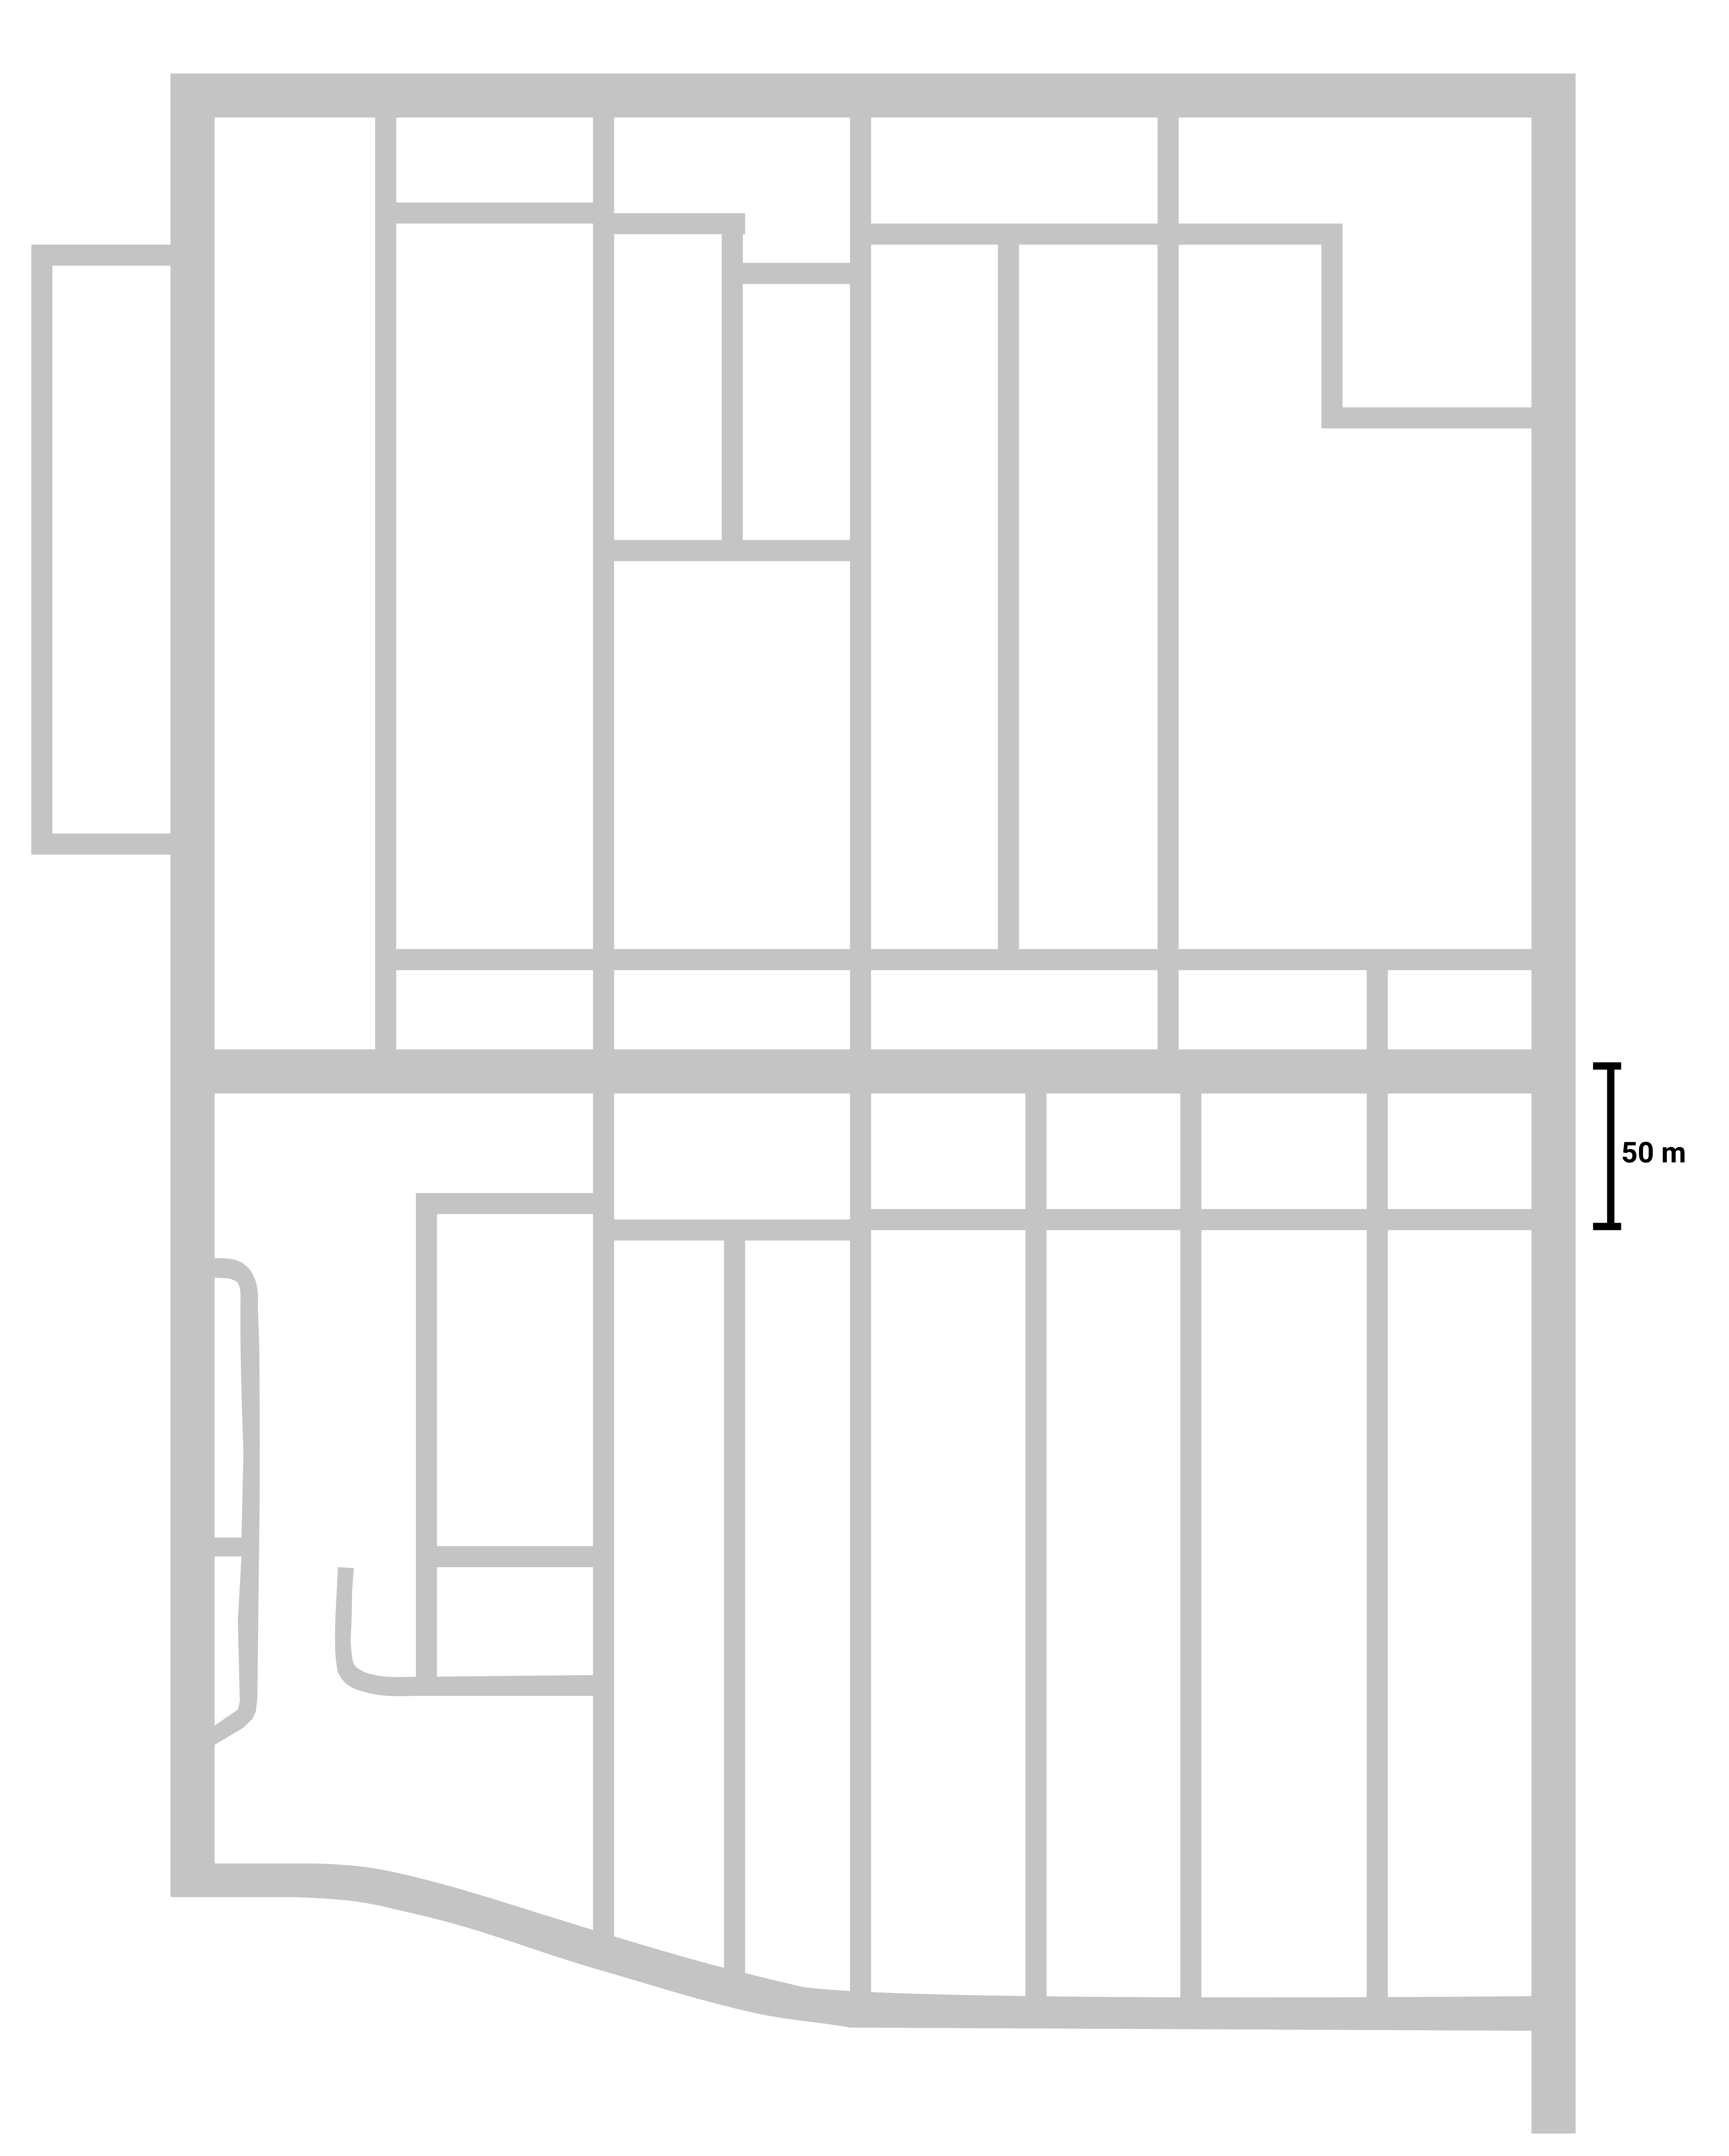
\includegraphics[width=\linewidth]{road_segment_outline}
		\caption{An example of a simulated road segment.}
		\label{fig:road_segment_outline}
	\end{figure}

	\subsection{Road Design \& Traffic Attributes}
		To create realistic urban scenarios, we based the road design of our experiments on popular road segments within Toronto, Ontario, sourced from OpenStreetMap, and the default traffic attributes on historic data sourced from Toronto OpenData, such as the number of vehicles on the road, traffic flow, average speeds, and many more. The city of Toronto was chosen for the models as it is the closest city to the author with significantly high levels of daily traffic flow.
	
		An example of an ideal road segment, as shown in Figure ~\ref{fig:road_segment_outline}, would include a network of high-volume intersections with multiple interlaced side roads that could potentially alleviate the pressures from the primary traffic flow.
	
	
	\subsection{Vehicle Models}
		We designed four vehicular models, including (1) ordinary civilian vehicles, (2) connected civilian vehicles, (3) ordinary ER vehicles, and (4) connected ER vehicles. The models vary in behavioural properties, physical properties, and technological capabilities. For instance, connected vehicles can communicate with our cloud server and between each other using V2V technology. ER models can exceed speed limits, run through red lights, and yield nearby traffic.

\section{Data Collection Methods}
	The experimental data recorded by the SUMO simulator is exported to a local database for later aggregation and analysis with the exported data from the cloud database. The data is broken into two parts:
	\begin{enumerate}
		\item Road-centric measurements for all vehicles passing through this segment include average speed, traffic flow, capacity, density, average headway, total risk score, and events such as near collisions, congestion, and traffic signals.
		\item Vehicular-centric measurements for each vehicle include speed, acceleration, path, delays, frequency of path modification, and frequency of detected ERs.
	\end{enumerate}
 	This list is not exhaustive and will be modified as the author grows familiar with the simulation software.
	

\section{Software \& Technology Related Design}

	\begin{figure}
		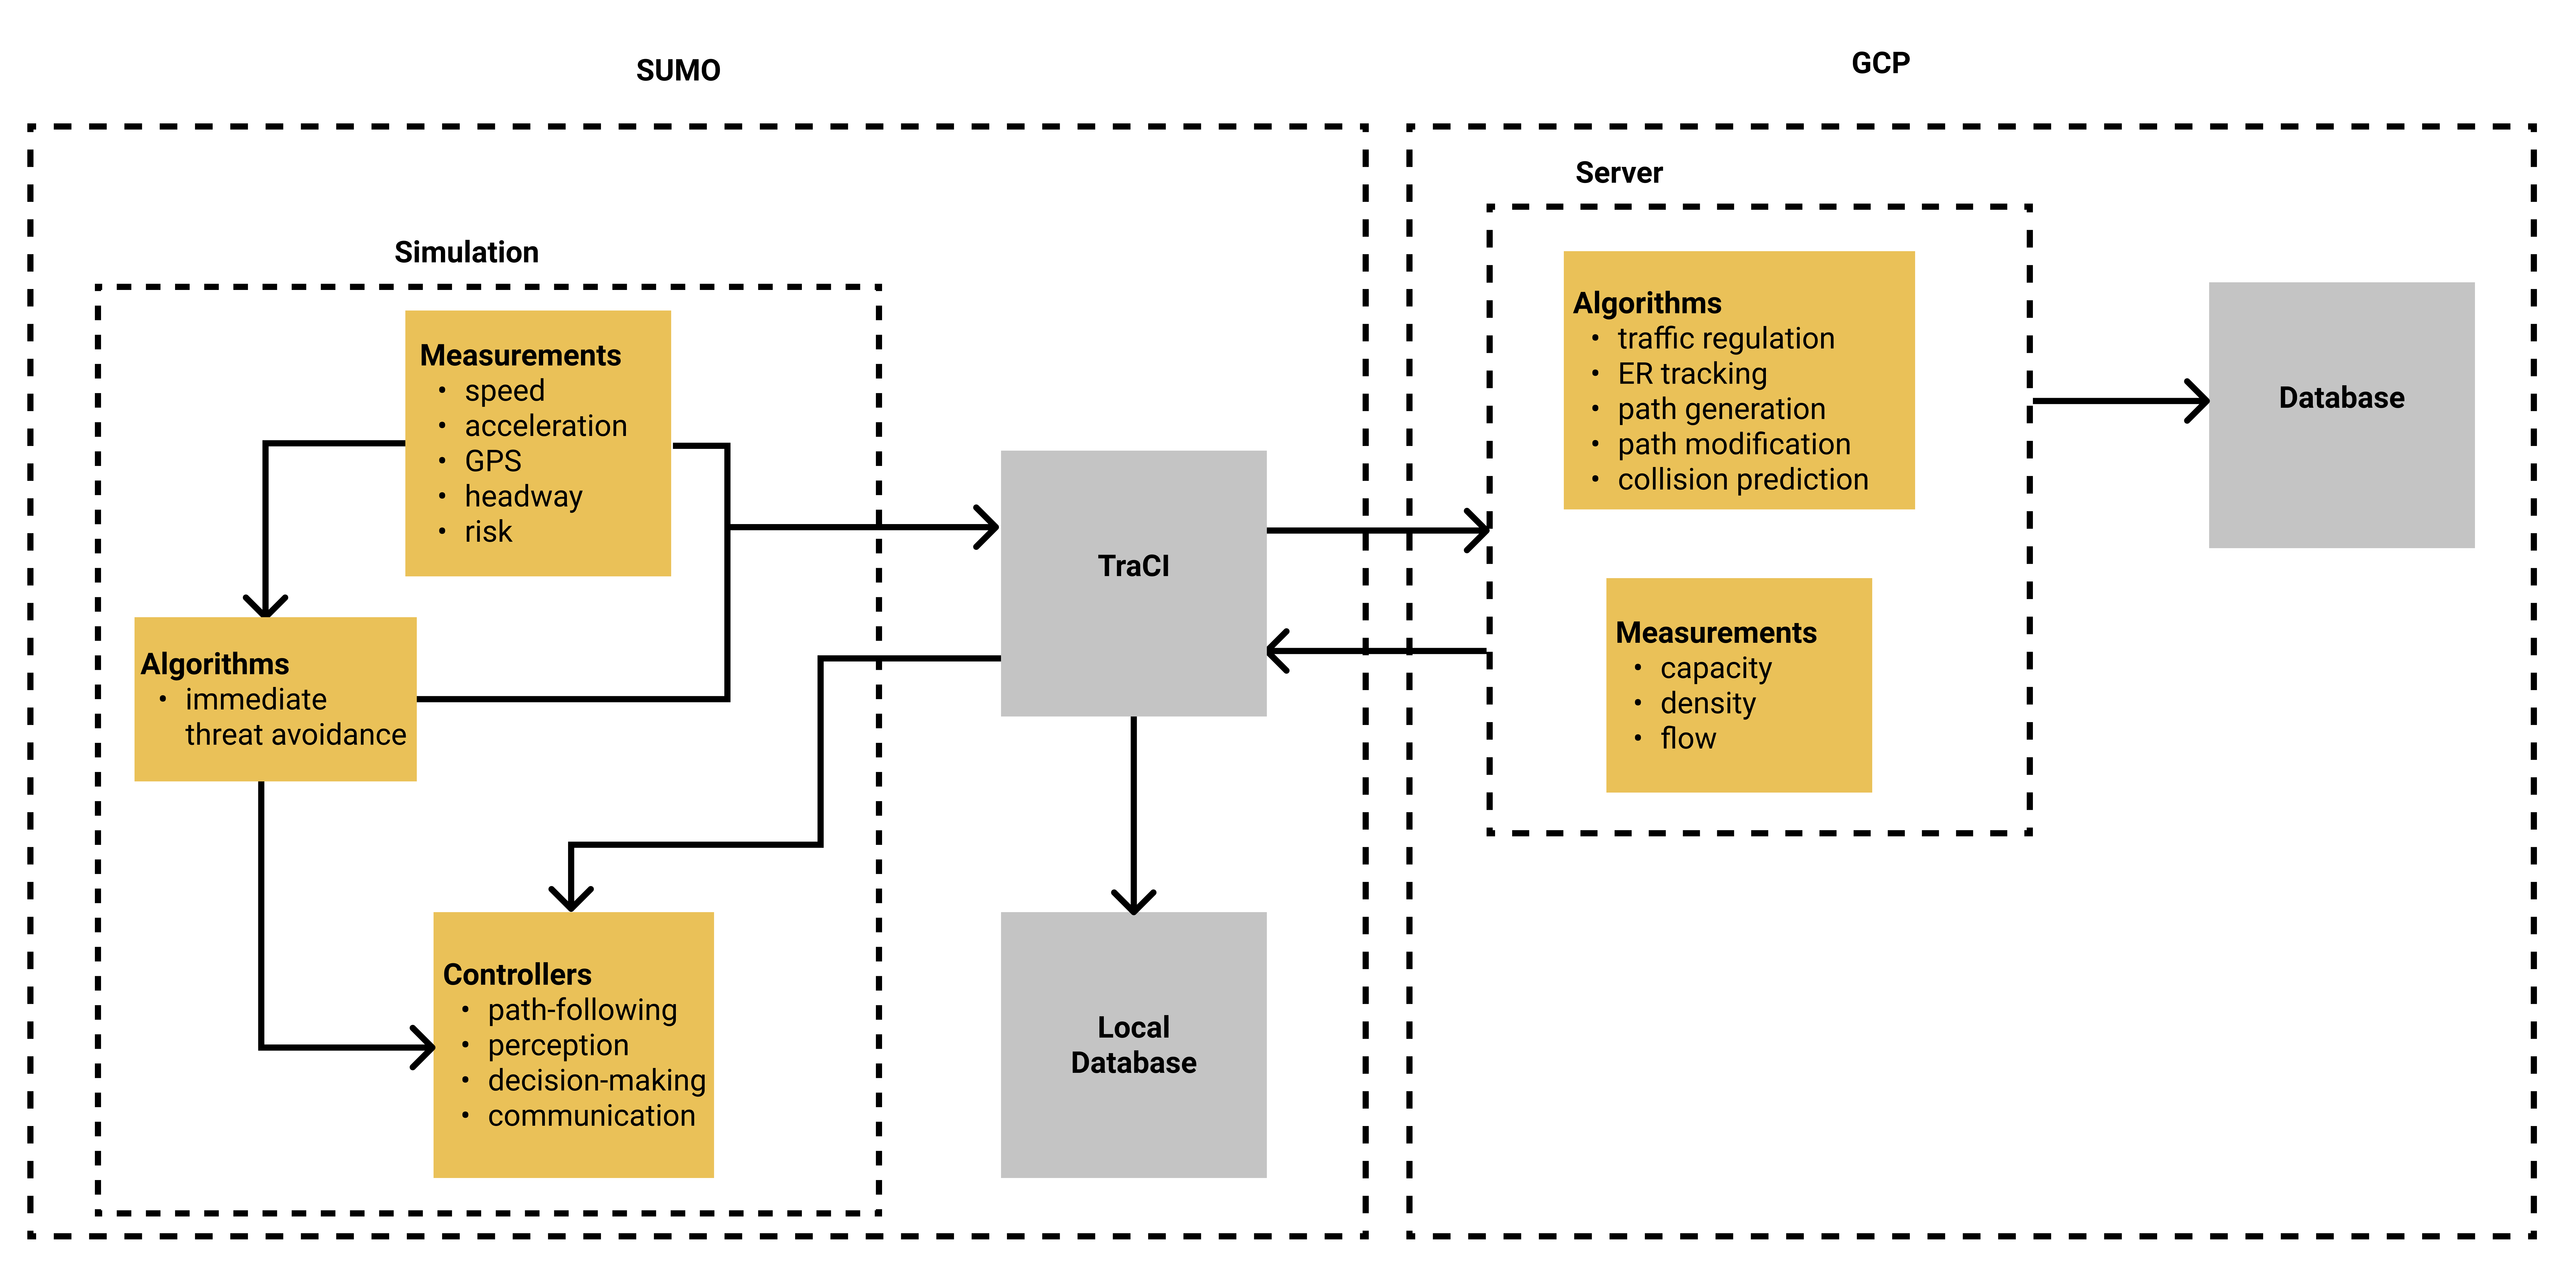
\includegraphics[width=\linewidth]{software_system_design}
		\caption{Software System Design Diagram.}
		\label{fig:software_system_design}
	\end{figure}
	
	As illustrated in Figure ~\ref{fig:software_system_design}, the system is comprised of two major components:
	\begin{enumerate}
		\item the simulator component (on the left);
		\item the cloud component (on the right).
	\end{enumerate}

	\begin{figure}
		\includegraphics[width=\linewidth]{vehicle_processing}
		\caption{Flowchart of onboard vehicle processing.}
		\label{fig:vehicle_processing}
	\end{figure}

	\begin{figure}
		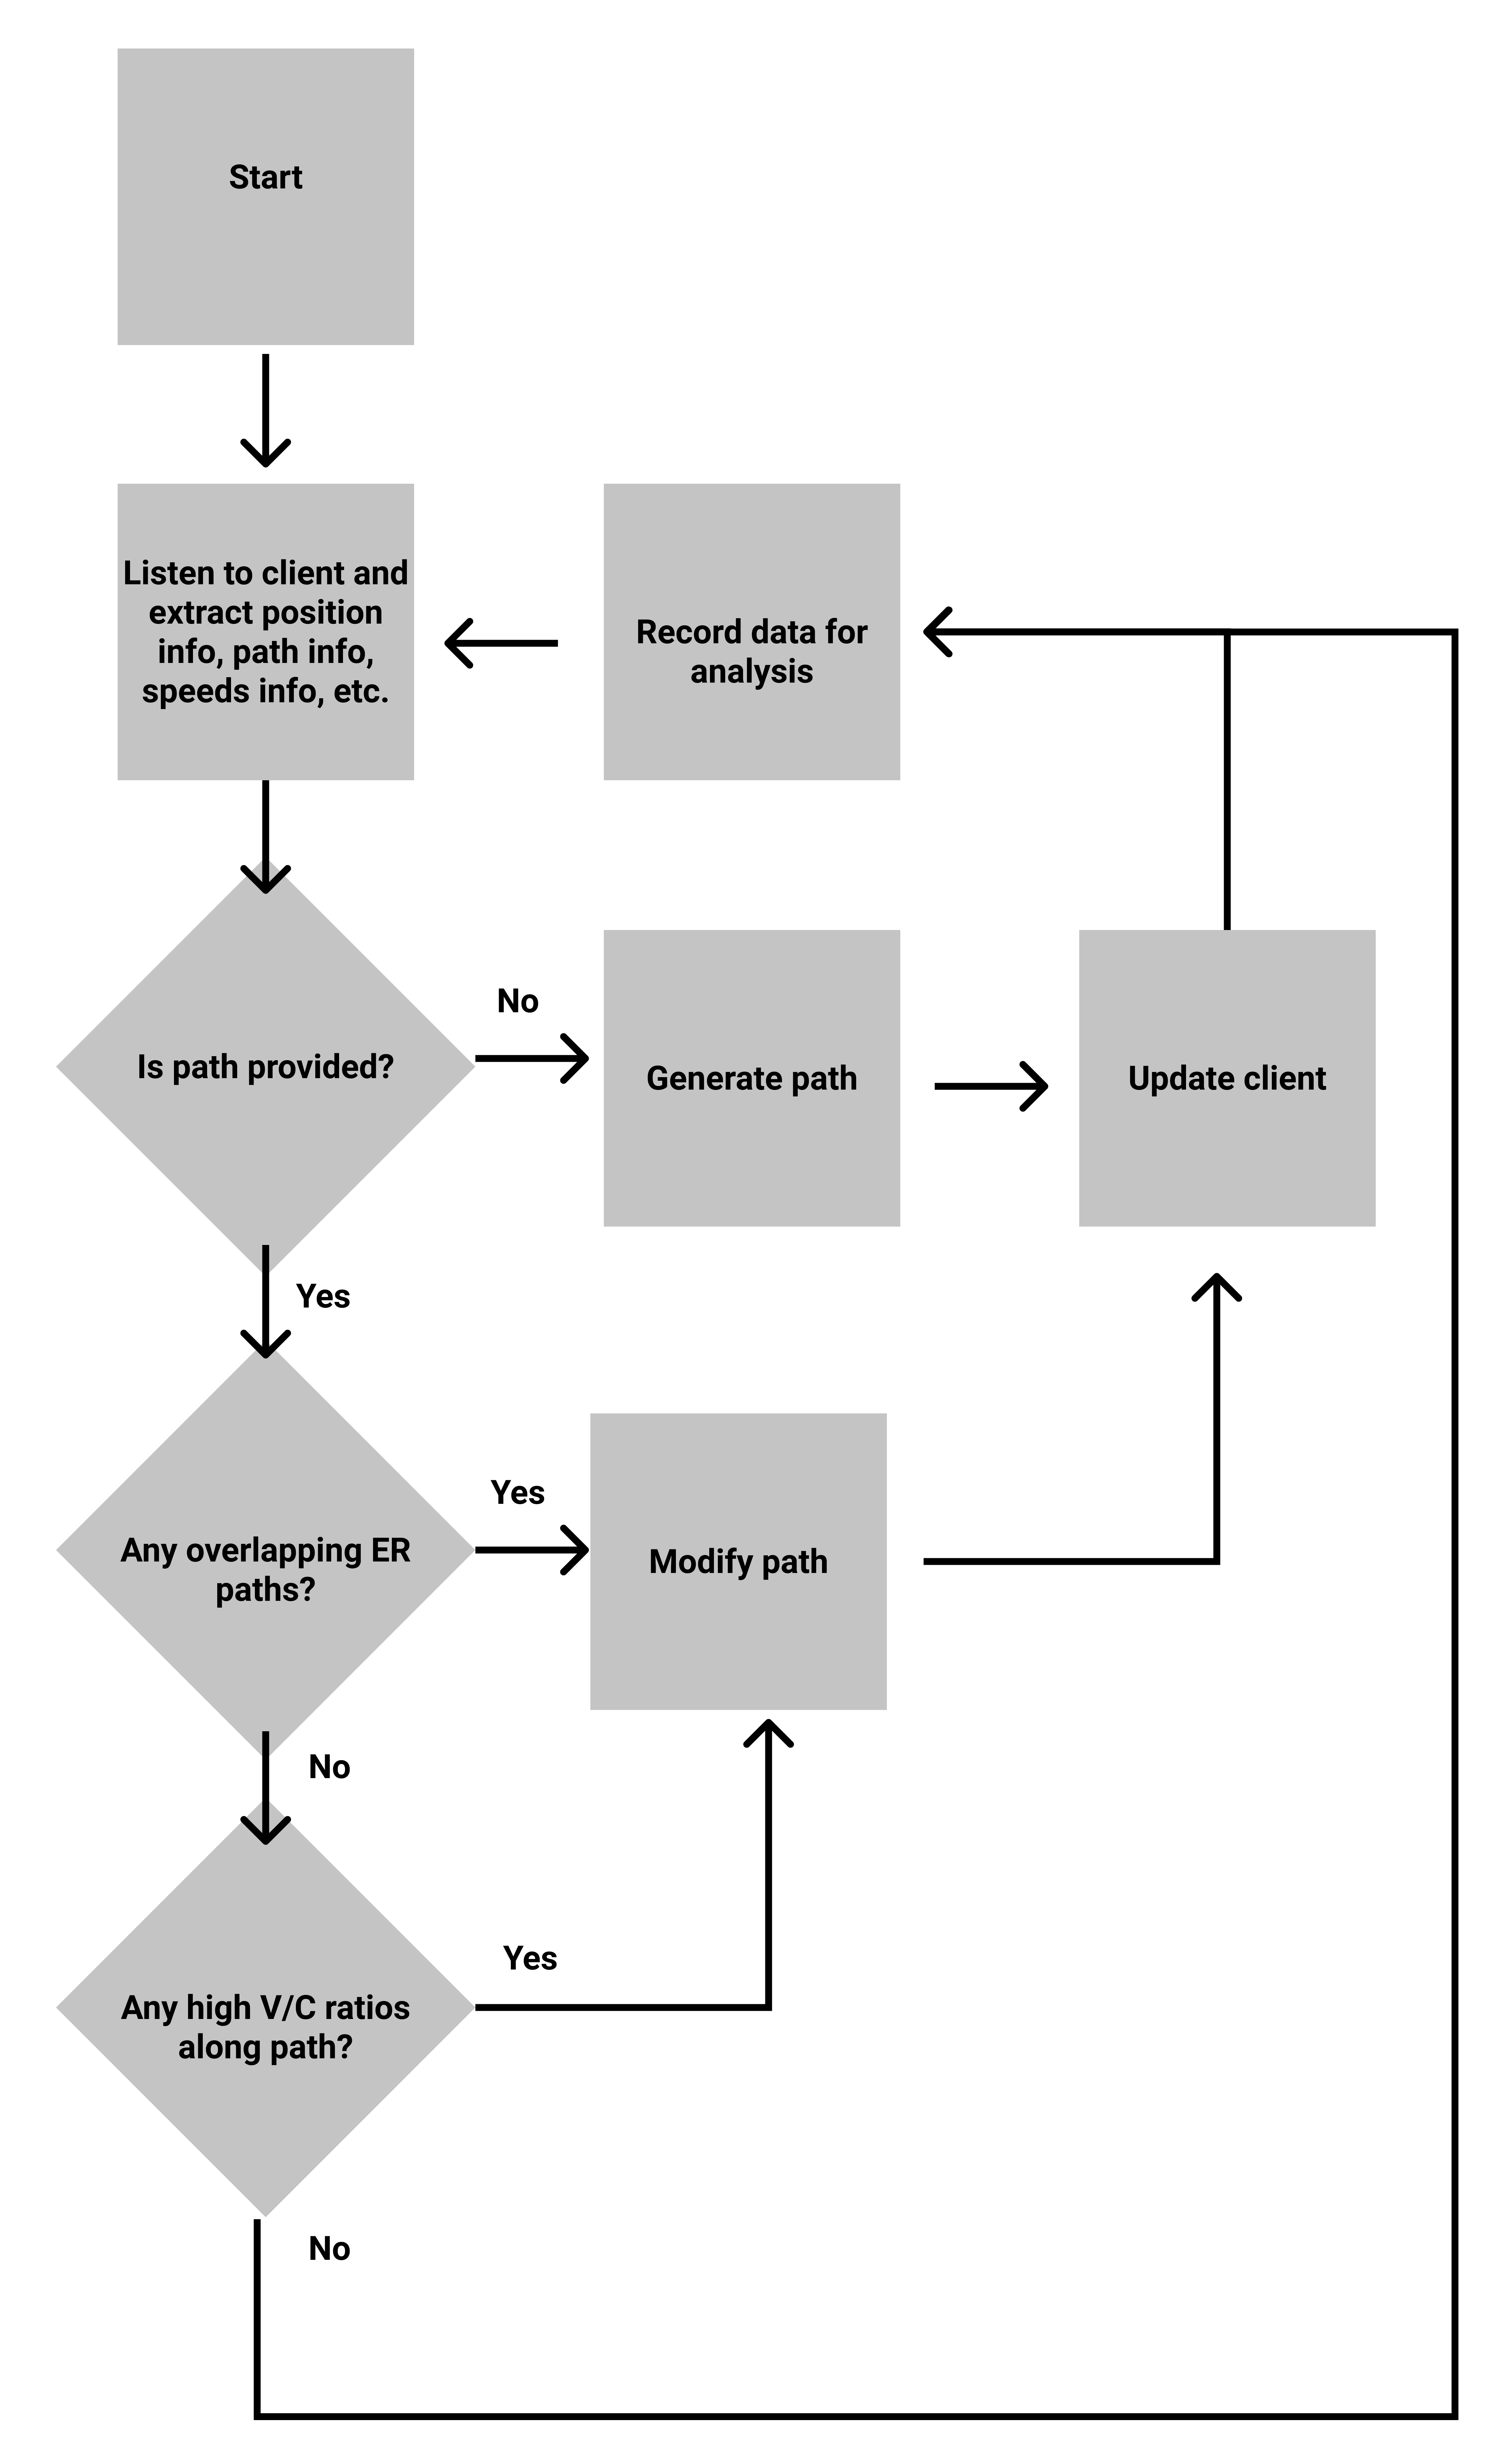
\includegraphics[width=\linewidth]{server_processing}
		\caption{Flowchart of cloud-based processing.}
		\label{fig:server_processing}
	\end{figure}

	The SUMO simulator software manages the simulation component and offers various tools for importing data, designing models, designing networks, and tracking data. A running simulation will continuously measure and compute a wide range of road and vehicular-centric data. The data feeds into the algorithms and controllers sub-components for localized risk assessment and decision-making such as slowing down, turning, and lane changing, as shown in the flowchart of Figure ~\ref{fig:vehicle_processing}. The simulator records the data in a local database for later analysis. The data and controllers within a running simulation can be read and manipulated in real-time through SUMO's TraCI middleware, empowering cloud computing. 

	The cloud server facilitates safer, smoother, and faster traffic for connected vehicles. The flowchart shown in Figure ~\ref{fig:server_processing} describes the relationship between the array of processes that this server is responsible for, including:
	\begin{enumerate}
		\item Path Generation
		\item Prediction of ER Path Collision
		\item Path Modification
	\end{enumerate}

	\subsection{Path Generation}
		\begin{figure}
			\includegraphics[width=\linewidth]{a-star_algorithm}
			\caption{Generated Path for an ER.}
			\label{fig:a-star_algorithm}
		\end{figure}
	
		
		This process is the first to be executed for every new client initiating their commute. It considers the client's current location, desired destination, and current traffic data to generate a path optimized for the lowest arrival time (i.e., fastest commute) using the A* algorithm. Figure ~\ref{fig:a-star_algorithm} depicts a minimalistic road segment with a path generated for an ER between two points.
		
	\subsection{Prediction of ER Path Collision}
		\begin{figure}
			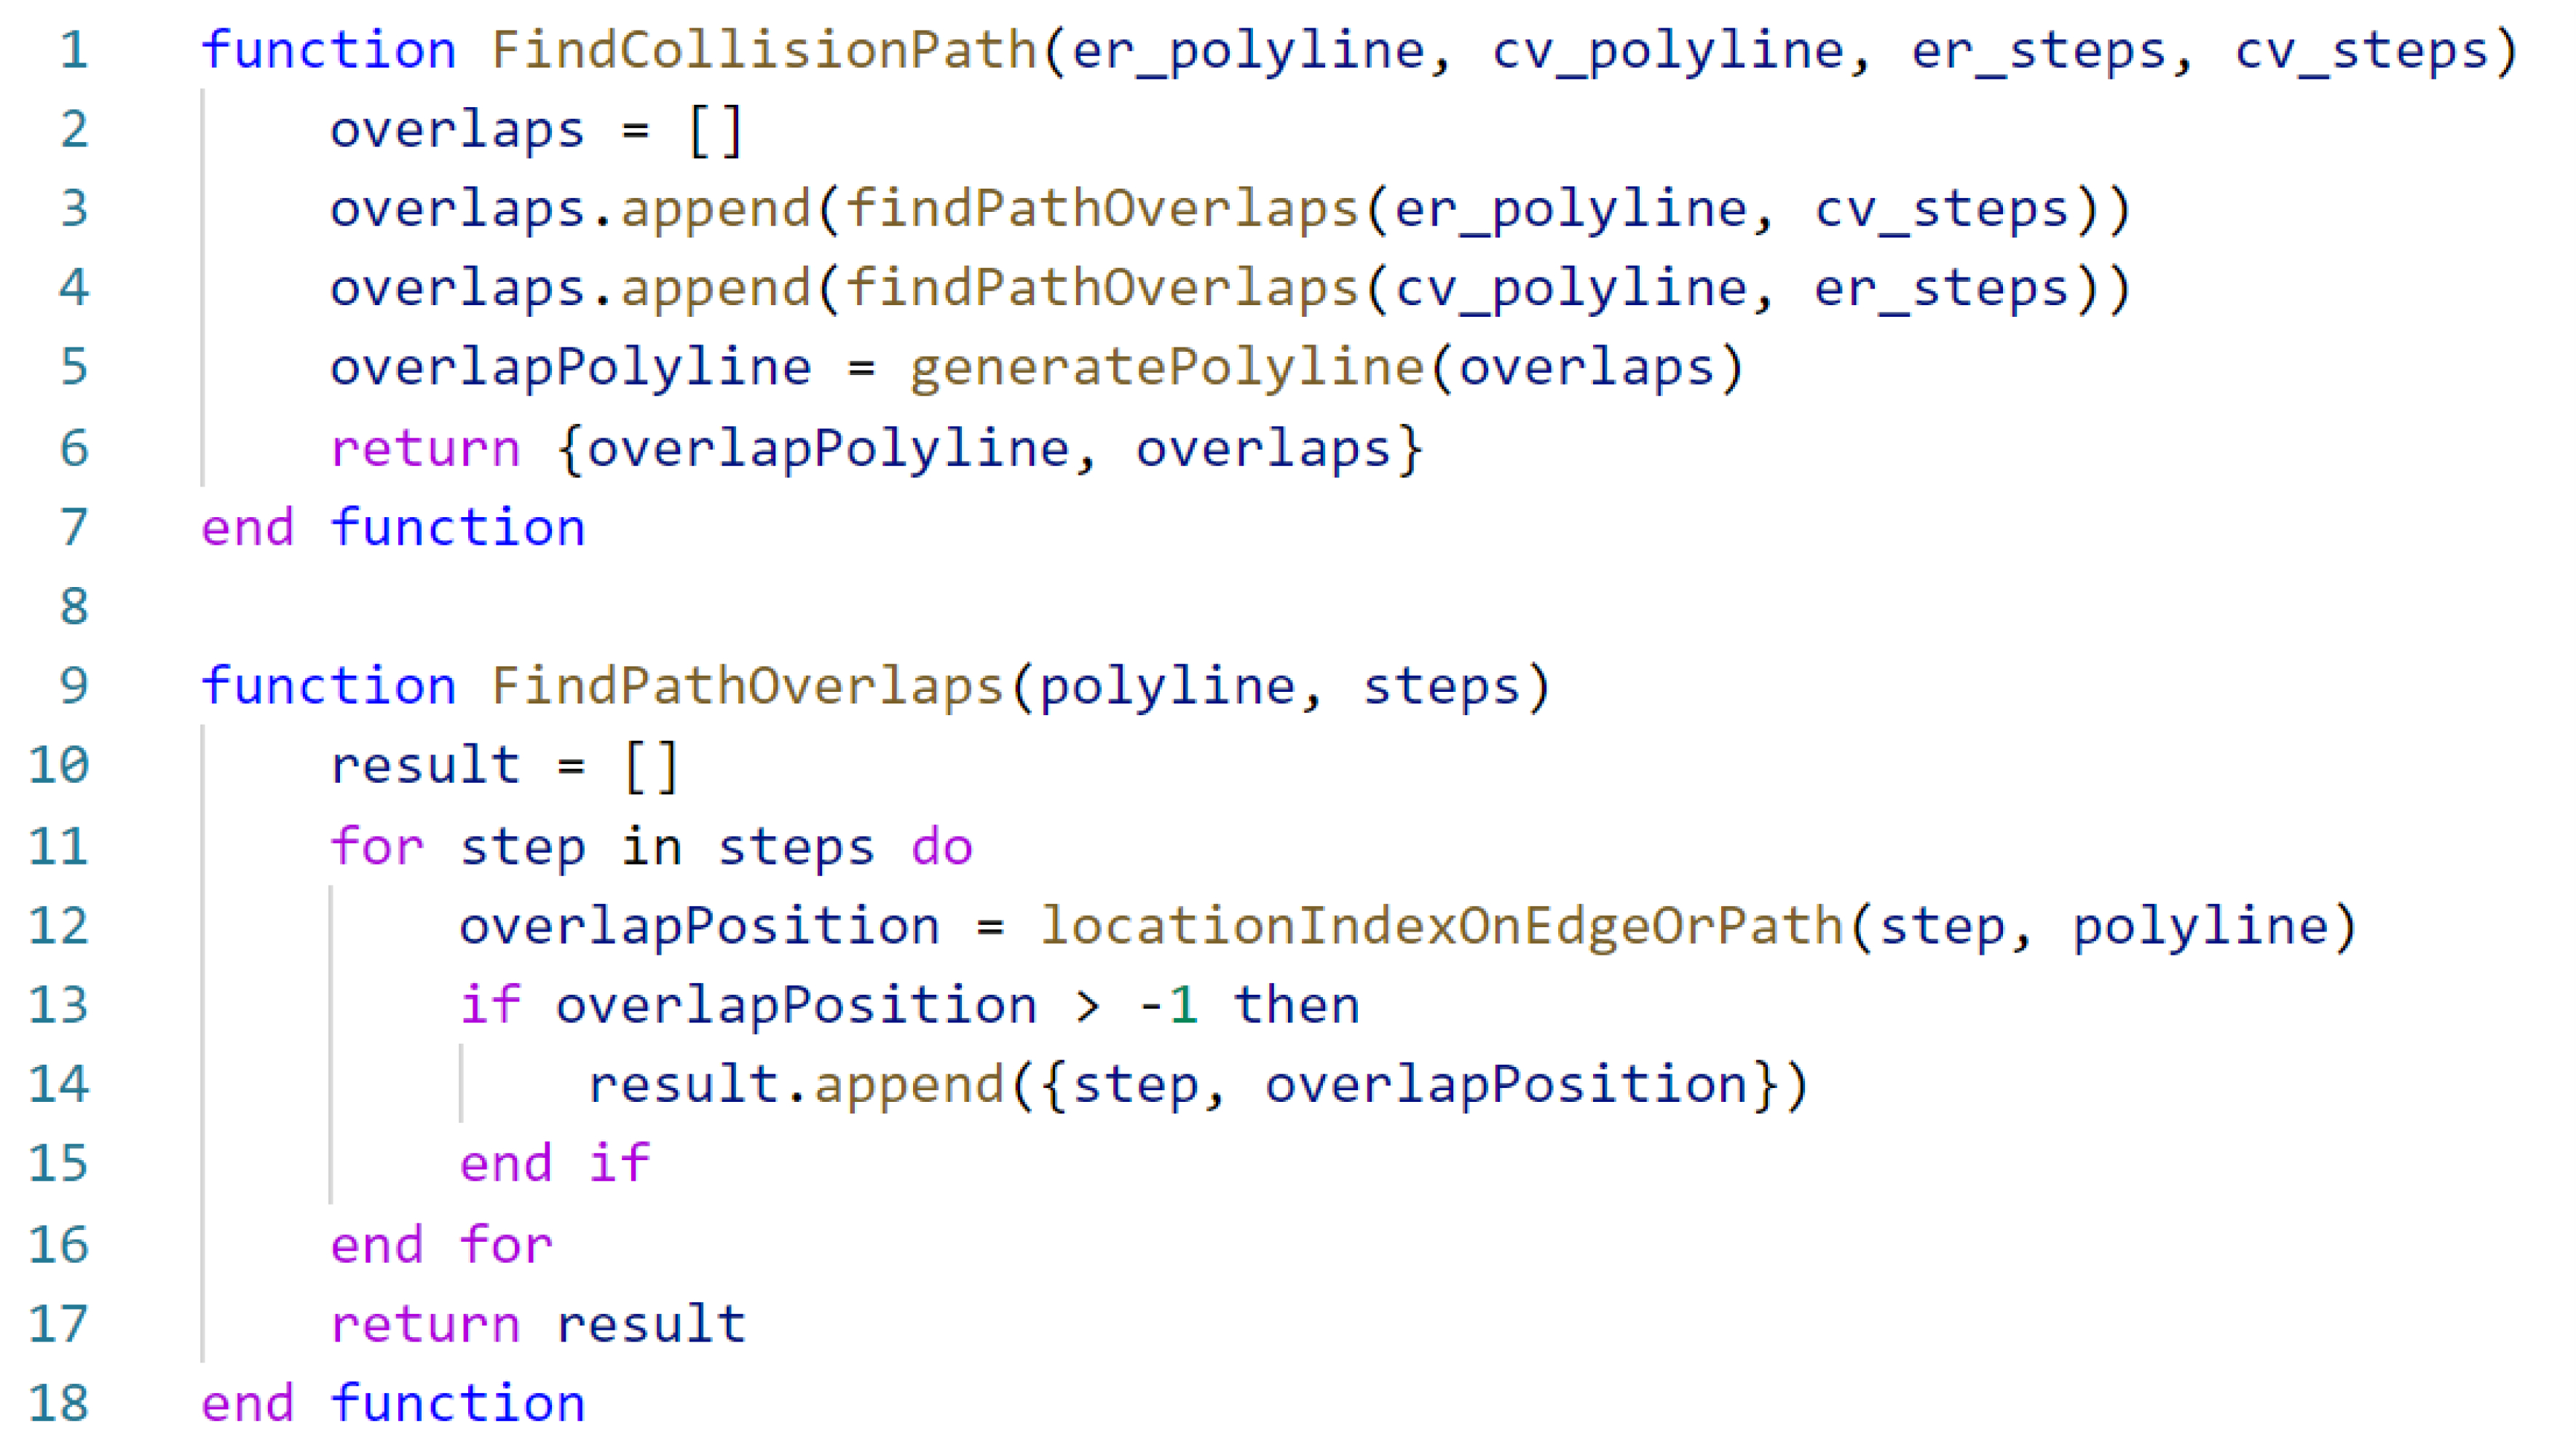
\includegraphics[width=\linewidth]{algorithm_01_psuedocode}
			\caption{Pseudocode for path collision detection between the routes of an \acrshort{ER} and civilian vehicle.}
			\label{fig:algorithm_01_psuedocode}
		\end{figure}
		
		\begin{figure}
			\includegraphics[width=\linewidth]{algorithm_01_diagram}
			\caption{Illustration of the path collision detection algorithm between the routes of an \acrshort{ER} and civilian vehicle.}
			\label{fig:algorithm_01_diagram}
		\end{figure}
	
		This process predicts when and where a connected civilian vehicle might collide with an active ER. The pseudocode in Figure ~\ref{fig:algorithm_01_psuedocode} elaborates on detecting all possible collision points along the paths of these two vehicles, and Figure ~\ref{fig:algorithm_01_diagram} provides a visual demonstration.
	
	\subsection{Path Modification}
		\begin{figure}
			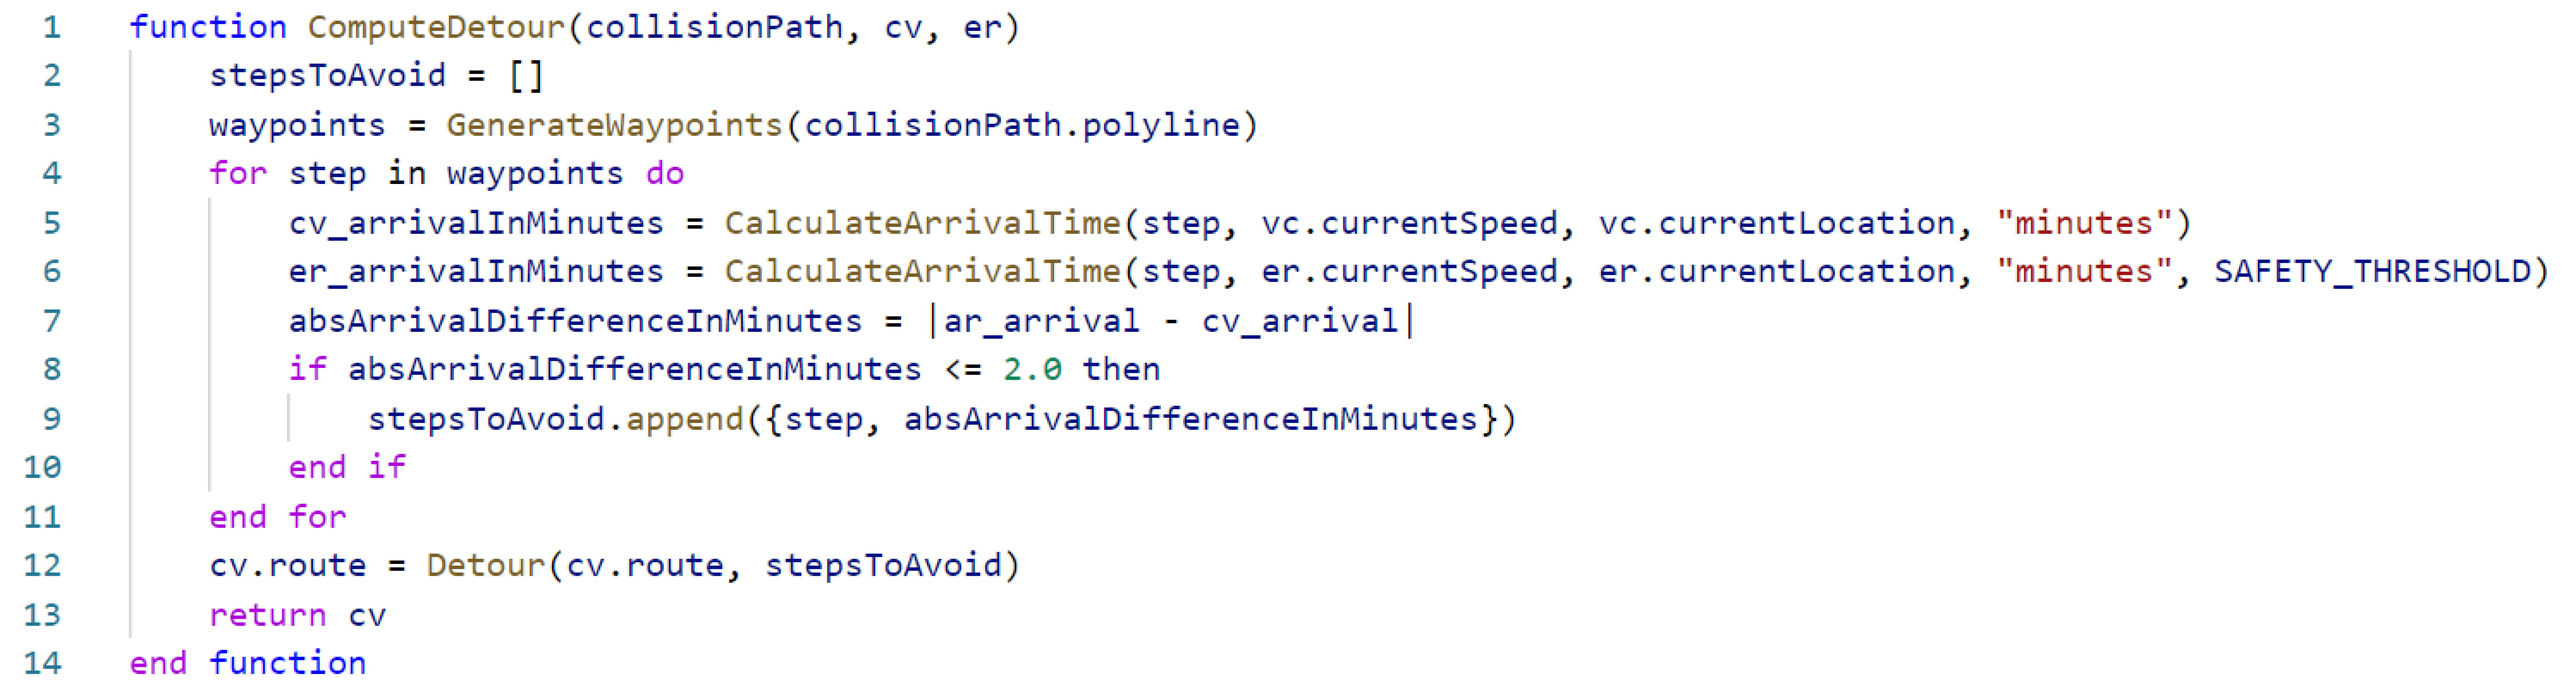
\includegraphics[width=\linewidth]{algorithm_02_psuedocode}
			\caption{Pseudocode for collision avoidance algorithm.}
			\label{fig:algorithm_02_psuedocode}
		\end{figure}
		
		\begin{figure}
			\includegraphics[width=\linewidth]{algorithm_02_diagram}
			\caption{Illustration of the collision avoidance algorithm.}
			\label{fig:algorithm_02_diagram}
		\end{figure}
		
		\begin{figure}
			\includegraphics[width=\linewidth]{ER_heatmap}
			\caption{A visual representation of the difference in traffic volume before (b) and after (b) the path modification process was applied.}
			\label{fig:ER_heatmap}
		\end{figure}
		
		In the event that the above process predicts a likely collision, this process is responsible for modifying the connected civilian vehicle's path to avoid roads where the collision is predicted to occur. Figure ~\ref{fig:algorithm_02_psuedocode} and Figure ~\ref{fig:algorithm_02_diagram} describes using the time-to-collision equation as a benchmark for comparing arrival times for both vehicles and deciding where the optimal path modification should occur. 
		Figure ~\ref{fig:ER_heatmap} depicts an example situation where a connected ER's path overlays high traffic volume roads (section b) and how this process evenly displaces localized traffic along side-roads (section a). You should notice the roads overlaying the ER's path (denoted with a dotted black line) change from a red color (high traffic volume) to a green color (low traffic volume). 


\section{Comprehensive Experiment Framework}
	\begin{figure}
		\includegraphics[width=\linewidth]{traffic}
		\caption{Stabilized traffic flow and volume of a road segment.}
		\label{fig:traffic}
	\end{figure}

	It is the law that all civilian drivers must adhere to proper protocol when nearby an \textit{active \acrshort{ER}}, such as slowing down, moving over, and halting until the \acrshort{ER} is a safe distance away (i.e., 150 meters away) \cite{MoveOver_2021, MTO_2020}. Our system helps connected civilian vehicles identify active \acrshort{ER}s sooner, with greater context, and helps avoid route collisions with them.  At the start of every experiment, as also done in \cite{Rizvi2007, Bahaaldin2017}, we allow the simulation to run for a consistent but arbitrary amount of time (e.g., 2 minutes), allowing the default background traffic to distribute evenly throughout the road segment. As illustrated in Figure ~\ref{fig:traffic}, the primary roads are expected to have significantly higher traffic volume (shown in red) than secondary roads (shown in green), as per the status quo of ordinary vehicles. After the calibration period, the average speeds, accelerations, and flow should level out should be constant, at which time we can apply any event or variable changes for this experiment, and its effects will be observed. 
	
	\begin{figure}
		\includegraphics[width=\linewidth]{locations}
		\caption{Example location of a road segment.}
		\label{fig:locations}
	\end{figure}

	Each experiment tests how road safety and arrival times are affected by variables such as, but not limited to, the penetration rates of connected vehicles, the number of active connected and ordinary ERs, the number of total vehicles, and origin and destination of ERs. Figure ~\ref{fig:locations} does not accurately depict an actual road segment or how location points are placed. It serves to simplify the demonstration of the underlying representation of each experiment.
	
	\textbf{Experiment 1:}
	Have the ER start in point A and travel to point C.
	This route represents a firetruck commuting from outside and through an urban road segment.
	
	\textbf{Experiment 2:}
	Have the ER start in point A and travel to point E, and after 2-minutes, return to corner A.
	This route represents an ambulance commuting outside and stopping within an urban road segment to retrieve a patient and return to the hospital outside the road segment.
	
	\textbf{Experiment 3:}
	Have the ER start at point E and travel to point A.
	This route represents a police vehicle parked within a road segment responding to a call outside. 
	
	\textbf{Experiment 4:}
	Have the ER start at point E, travel to point F, point A, and point C. 
	This situation represents a police vehicle car chase, starting within the road segment.


\section{Data Analysis Methods}
	Calculating traffic safety risk is a complex and ambiguous task. The authors of the \cite{leur_sayed_2002} developed a road safety risk index (RSRI), enabling a quantitative approach for measuring road safety. The RSRI is based on three isolated fundamental elements such as exposure, probability, and consequence.
	
	\( \text{RSRI} = \text{Exposure} \times \text{Probability} \times \text{Consequence} \)
	
	Where:
	\begin{itemize}
		\item Exposure = measure to quantify the exposure of road users to potential roadway hazards.
		\item Probability = measure to quantify the chance of a vehicle being involved in a collision.
		\item Consequence = measure to quantify the severity level resulting from potential collisions.
	\end{itemize}

	Alongside the RSRI parameters, we also consider several traffic parameters and processes known to influence traffic safety measured by proximal indicators. These include speed and speed variance, gap-acceptance in yielding situations, headway between vehicles in traffic streams, and traffic flow rates (including derived measures such as saturation and density). By tracking these various parameters over multiple road segments in different driving situations, we can analyze which parameters significantly impact road safety with varying connected vehicle penetration rates.
	
	\subsection{Exposure}
		Exposure is the measure to quantify the exposure of drivers to potential roadway hazards, such as nearby vehicles. It provides a score ranging from zero to a maximum of 3.0, with a high score representing high exposure.
			
			\( \text{Exposure}_\text{urban}=(\frac{V_{i(\text{major})} \times V_{i(\text{minor})}}{V_{\text{max}(\text{major})} \times V_{\text{max}(\text{minor})}})\times3.0 \)

		Where:
			\begin{itemize}
				\item \( V_{\text{max}(major)} \) = maximum volume on the major road.
				\item \( V_{\text{max}(minor)} \) = maximum volume on the minor road.
				\item \( V_{i} \) = volume at the location of a specific roadway.
			\end{itemize}

	\subsection{Consequence}
		Consequence is the amount of danger the driver can incur if an accident were to happen. It is a ratio between the posted speed and maximum posted speed of a roadway segment. Maximum posted speed can equal the posted speed, or it can be based on a larger area. It provides a score ranging from zero to a maximum of 3.0, with a high score representing high consequence.
		
		\( \text{Consequence}=(\frac{\text{Posted Speed}_i}{\text{Posted Speed}_\text{max}})\times3.0 \)
			
		Where:
			\begin{itemize}
				\item \( \text{PS}_i \) = posted speed at the location of a specific roadway.
				\item \( \text{PS}_\text{max} \) = maximum posted speed.
			\end{itemize}

	\subsection{Volume-to-Capacity Ratio}
		Volume-to-Capacity (V/C) is the ratio of current or projected demand flow rate to the capacity of a segment. It is an indicator of how close a roadway is operating to its capacity. An increase in the V/C ratio indicates longer vehicle delays and queuing.
		
		\( \text{V/C Ratio}=\frac{\text{Demand flow rate}}{\text{Capacity}} \)
		
		Where:
		\begin{itemize}
			\item Demand flow rate = volume of vehicles on a transportation facility (vehicles per hour per lane) for a given segment length.
			\item Capacity = the maximum number of vehicles a transportation facility can handle (veh/hr/ln) for a given segment length.
		\end{itemize}
	
	\subsection{Headway}
		Headway is the time difference between successive vehicles as they pass a point or segment, measured from the same point on each vehicle, expressed in seconds per vehicle.
		
		\( \text{Headway}=\frac{\text{Spacing (ft/veh)}}{\text{Speed (ft/sec)}} \)
		
	\subsection{Traffic Speed}
		The average speed of all vehicles passing through a point or segment. Variations in the speed of vehicles within and across lanes are important traffic safety indicators.
		
		\( v_t=\frac{1}{n}\sum^{n}_{i=1}{v_i} \)
		
		Where:
		\begin{itemize}
			\item \( v_t \) is the time mean speed.
			\item \( v_i \) is the spot speed of \(i^{th} \) vehicle.
			\item \( n \)is the number of vehicles observed.
		\end{itemize}
		
	
\section{Research Validation}
	To combat any uncertainty that the observed results are the result of our system, the following steps were taken:
	\begin{itemize}
		\item The simulations are generated using time seeds. This enables reproducible situations where causative factors for the results can be validated.
		\item Every experiment is run with varying levels of connected vehicle penetration rates. This is done to verify whether the obtained results in the situation were a result of the connected vehicles; increasing the number of connected vehicles should amplify the results.
	\end{itemize}


\section{Assumptions \& Limitations of the Study}
	Human drivers are prone to make mistakes in following a provided path due to distracted drivings or unforeseeable circumstances in the real world. To reduce the complexity of our simulations, we assume that our connected vehicle drivers follow the paths provided 100\% of the time. We also do not consider any weather conditions, pedestrians, or non-car road users. We limit the size variations of our vehicle models to one average sedan for civilian drivers and an average firetruck, ambulance, and police car.


\section{Summary}
	In this chapter, we described the design and rationale of the experiments' setup, defined the system architecture design and data collection processes, explained the various experiment scenarios, explaining how the results will be used to validate our research, and highlighted any assumptions and limitations.
